\chapter{工作笔记}
\section{转写数据训练}
\subsection{准备数据}
首先对数据进行清洗,期间碰到的坑数不胜数,防不胜防。

kaldi训练的时候,在数据准备阶段,需准备以下这些文件:
\begin{itemize}
	\item wav.scp: 格式为 \textcolor{gray}{"<index> <wave\_path>"},存储着音频的索引和绝对路径;
	\item segments: 格式为\textcolor{gray}{"<subindex> <index> <start\_time> <end\_time>"},存储着音频所对应的segments的子索引,原始音频索引和起止时间点(秒)。
	\item text: 格式为\textcolor{gray}{"<subindex> <word1> <word2> ..."},存储着segment的索引和对应的文本;
	\item utt2spk: 格式为\textcolor{gray}{"<subindex> <spk>"},存储着segment的索引及其所对应的说话人;
	\item spk2utt: 格式为\textcolor{gray}{"spk <subindex1> <subindex2> ..."}。
\end{itemize}

说明一下,一个原始音频中,不一定每个时刻都有人说话,所以我们可以得到有说话人说话部分的segments文件,这样kaldi在进行特征提取、对齐和chain model的训练的时候就只考虑那些segments了,省时省力省空间。如果没有segments文件,上述的"<subindex>"和"<index>"就是一样的了。如果有segments,那么相当于说用这些音频片段去进行对齐和训练,所以每个片段对应的文本和说话人都得有,所以text、utt2spk和spk2utt这些文件里面都是用的"<subindex>"。

在清洗数据的时候需要注意以下几点:
\begin{itemize}
	\item 音频格式要统一,我们需要的是8k,16-bit Signed Integer PCM的wav文件,所以通过sox或者FFmpeg都得进行转换;
	\item 注意待处理的文本格式,首先文本的编码方式可能不一样,其次不同的库文本标注的格式也不一样;
	\item 音频和文本不统一;
\end{itemize}

我们遇到的音频格式主要有:
\begin{itemize}
	\item WAV Sample Encoding: A-law
	\item WAV Sample Encoding: GSM
	\item WAV Sample Encoding: 16-bit Signed Integer PCM
	\item MP3
	\item PCM
	\item V3
\end{itemize}

那进行音频的格式统一之后,我们就可以得到 wav.scp,再对文本进行去大小写,去标点符号,去乱七八糟的符号之后,我们就可以得到text、segments、spk2utt和utt2spk了。在得到所有的上述文件之后,调用kaldi的脚本 utils/fix\_data\_dir.sh 来进行排序和去除无效的数据。

在处理的过程中,有一些需要注意的事情记录如下:
\begin{itemize}
	\item 在进行音频和文本匹配的时候,一定要保证音频名和文本名是匹配的,也就是说,如果找 test.txt 对应的音频,那么一定要保证该音频的名字是 test.wav;
	\item 转写文本中某一个segment标注了"有效"或者"valid",并不一定是真的有效,还得再看看那个segment对应的文本是不是空的,在进行文本清洗的时候,要判断下文本的长度是不是等于0;
	\item 音频的格式虽然是wav,但是它不一定是kaldi能处理的wav……比如上面提到的A-law和GSM,kalid就无法处理,而A-law用python的标准库 wave去读也读不了,所以A-law很好判断,但是GSM wave可以读……所以一定要保证音频格式的统一;
	\item 音频可能是双通道的;
	\item 音频可能头文件存储的音频长和实际长度不一样;
	\item 音频可能是损坏的……即全是噪声,频谱图趋于均匀分布,这种的可以考虑算下音频的RMS,如果RMS比正常音频大很多,那说明就是有问题的,因为噪声越大,RMS越大;
	\item 有的音频虽然以wav为后缀名,实际上人家是pcm;
	\item 限制变量的正负,比如segment的起止点,肯定是大于等于0的。
\end{itemize}

\subsection{准备词典和词表}
我们准备好了语音和文本,那如何将二者联系起来呢?简单来说,如图\ref{fig:basic-theory},HMM连接了音频特征和音素序列,而音频特征由原始音频提取得到,音素序列可以通过词典转换得到,因此词典是十分重要的。
\begin{figure}[h]
  \centering
  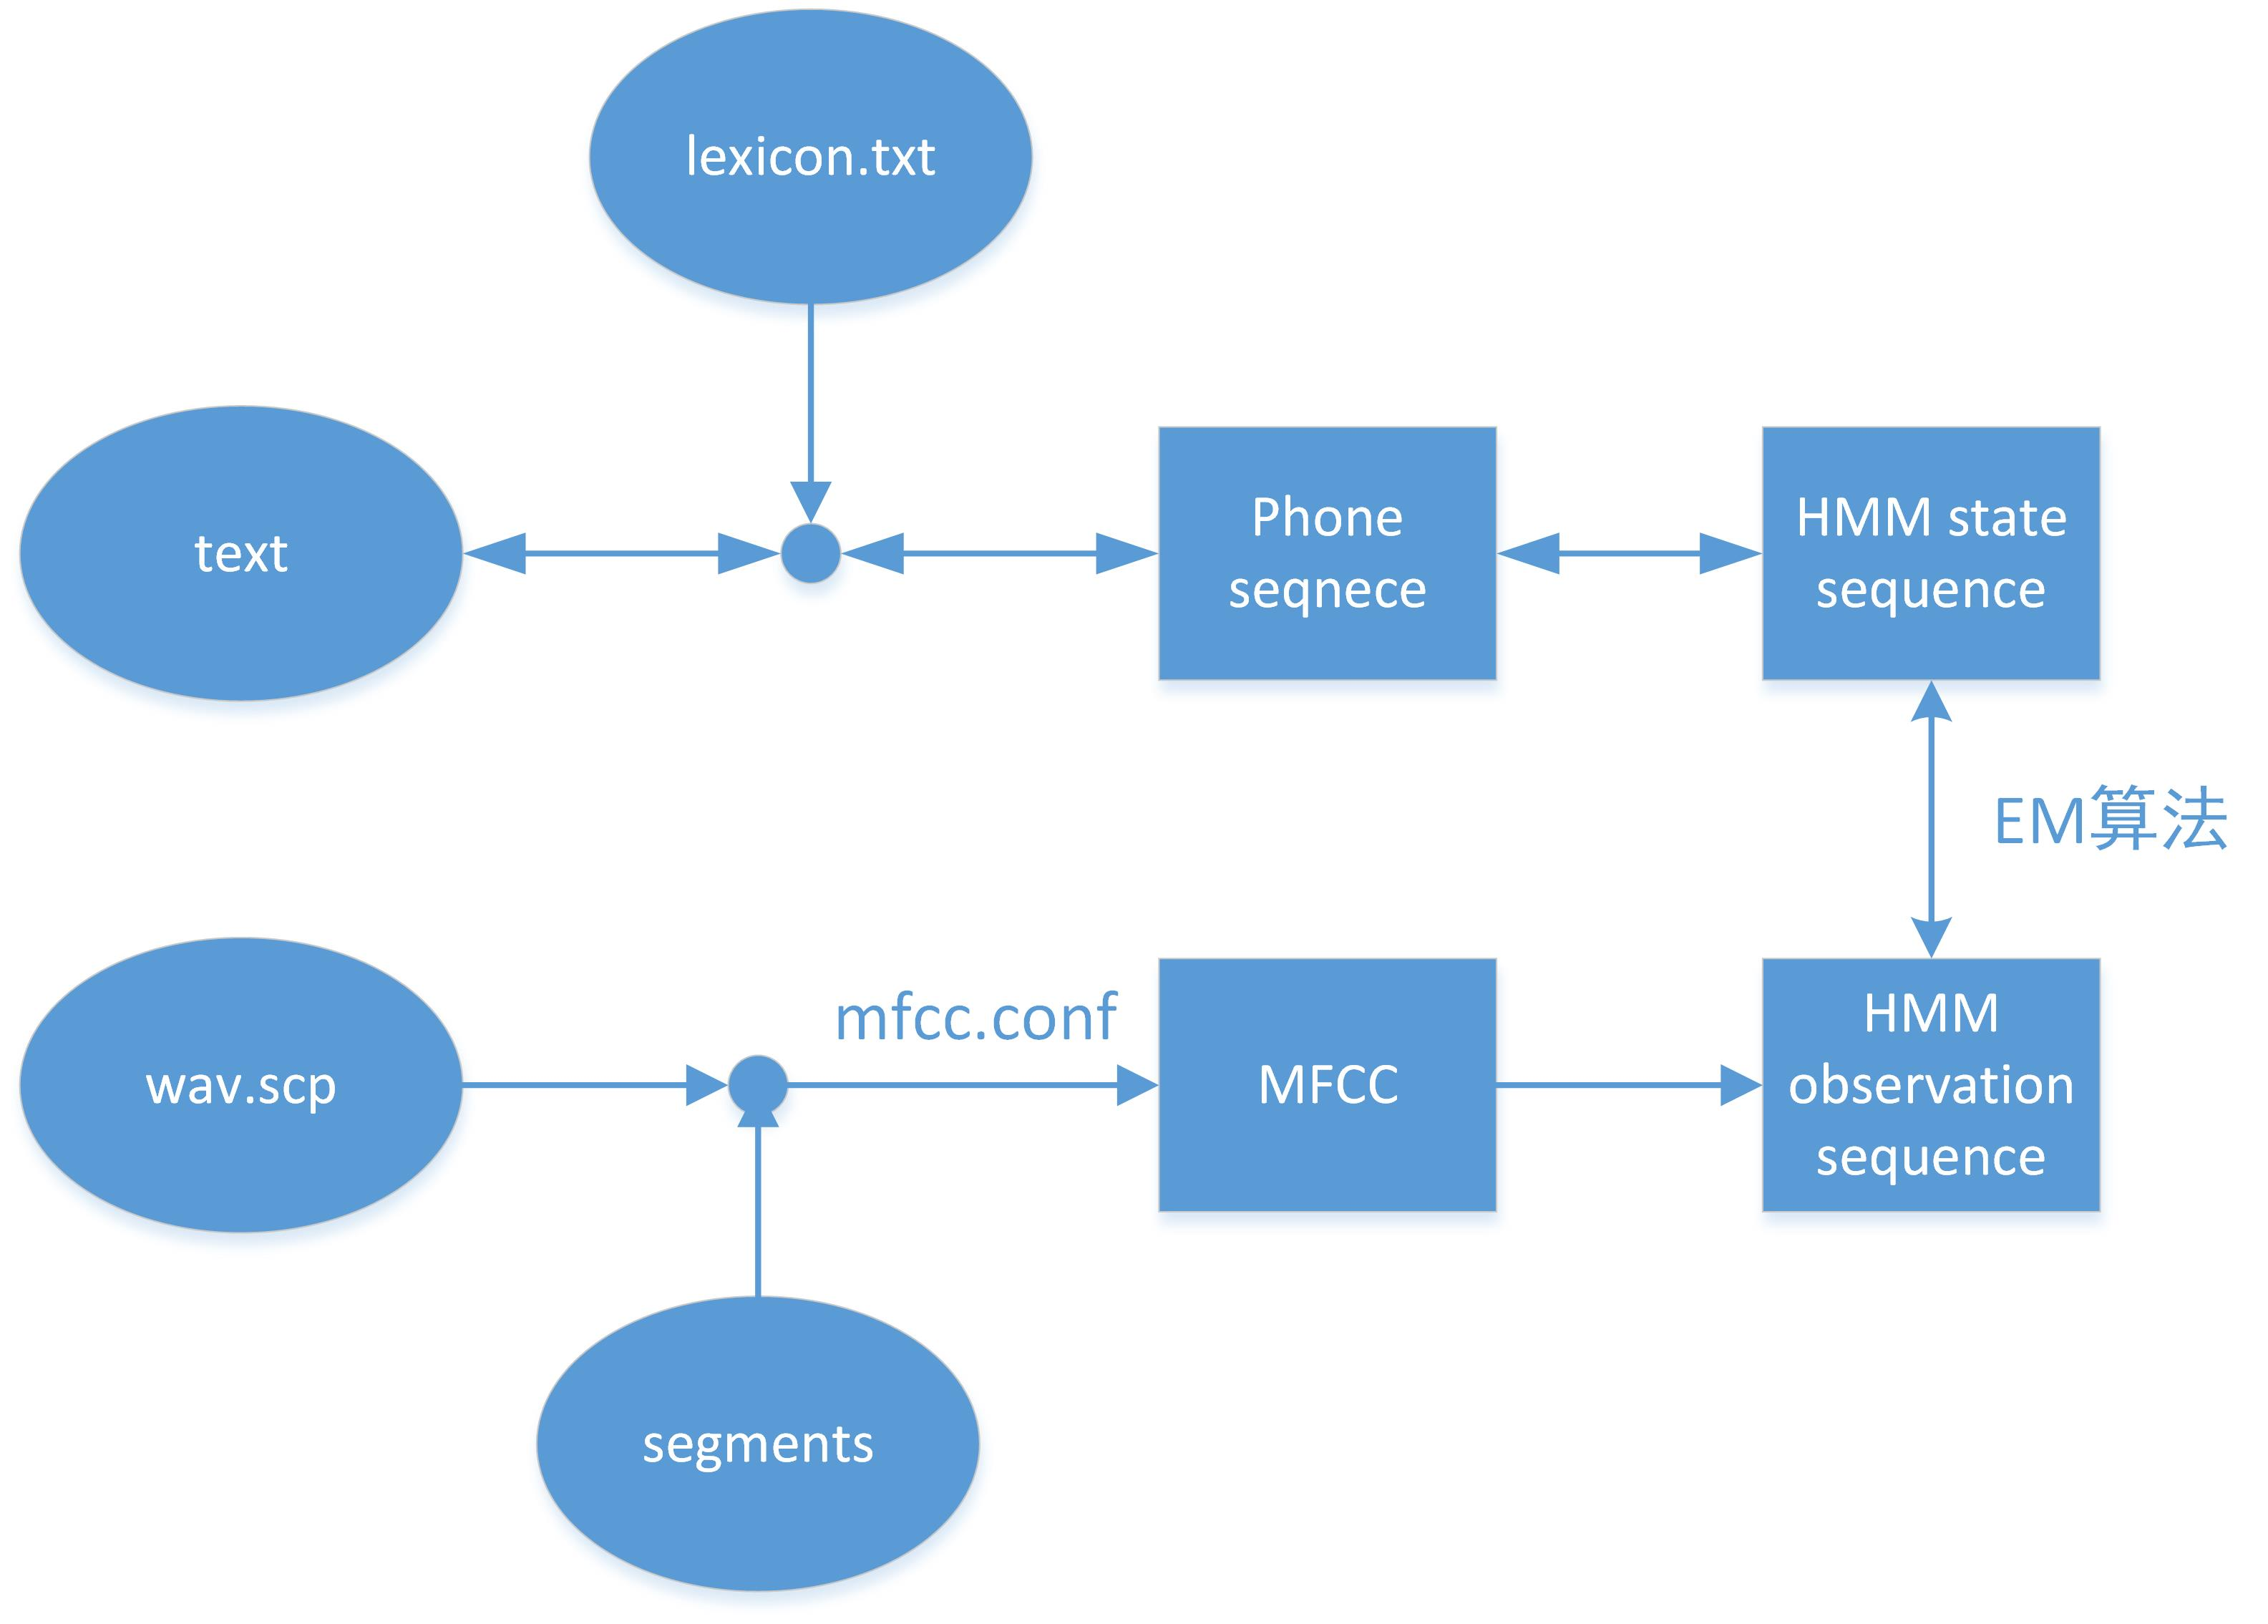
\includegraphics[width=0.7\textwidth]{chap1-1}
  \caption{原始音频和文本是如何连接起来的 \label{fig:basic-theory}}
\end{figure}

那么在准备词典之前,我们首先要知道整个数据集中有哪些词,所以首先我们要对所有的文本进行分词,在上面我们提到的 text 文件中,其实就已经是按照词的方式呈现出来了。比如说有句话的索引为A00001,其对应的文本是"我在吃饭",那么text文件中存储的格式就是:
\begin{lstlisting}[language=shell, numbers=left, 
         numberstyle=\tiny,keywordstyle=\color{blue!70},
         commentstyle=\color{red!50!green!50!blue!50},frame=shadowbox,
         rulesepcolor=\color{red!20!green!20!blue!20},basicstyle=\ttfamily]
A00001 我 在 吃饭
\end{lstlisting}

词典的格式为 \textcolor{gray}{"<word> <pronouciations>"}。

除却发音词典,词表(vocabulary)用于语言模型的训练,一般是N-gram。所以同样,我们还需要一个vocab.txt文件。其每一行都有一个word。

\subsection{开始训练}



\subsection{第一轮训练结果记录与分析}
经过第一轮训练之后,对提取的测试集进行解码,为了看不同语言模型下模型的性能,我们采用了四种语言模型去进行解码,这四种LM的特点如下:
\begin{itemize}
	\item 整个数据集包含的文本训练的LM,记作all-lm;
	\item 大语言模型测试的小语言模型,记作small-lm;
	\item 大语言模型进行rescore,记作big-rescore-lm。
\end{itemize}

经过这些不同的语言模型解码之后得到的CER结果如表\ref{tab:lm-decoder}。
\begin{table}[h]
 \centering
 \caption{不同语言模型解码的测试集CER}
	 \begin{tabular*}{1\textwidth}{@{\extracolsep{\fill}}ccccccc}
	 \toprule
		{\bf 语言模型} & {\bf 大小} & {\bf CE(\%)} &{\bf INS} &{\bf DEL}  &{\bf SUB} &{\bf Total}\\
	 \midrule
	   all-lm         &  83M   & 22.97   &   7420 &   22157 & 29619  & 257710 \\
	   small-lm       &  50M   & 28.45   &   7376 &   23291 & 42650  & 257710 \\
	   big-rescore-lm &  3.7G  & 27.58   &   7169 &   23825 & 40092  & 257710 \\
	 \bottomrule
	 \end{tabular*}%
 \label{tab:lm-decoder}%
\end{table}%

转写数据实际上由12个数据库组成,对每一个数据库单独统计CER,得到表\ref{tab:cer-per}。
\begin{table}[h]
 \centering
 \caption{不同语言模型解码的测试集CER}
	 \begin{tabular*}{1\textwidth}{@{\extracolsep{\fill}}ccccccc}
	 \toprule
		{\bf Project   } & {\bf ID   } & {\bf #WRDS   } & {\bf #SUB    } & {\bf #INS    } & {\bf #DEL    } & {\bf CER  } \\
	 \midrule
		TR2017097  &          5 &      15480 &       2416 &        361 &        552 &   0.215052 \\
		TR2018011  &         11 &       5511 &        716 &         87 &        161 &   0.174923 \\
		TR2018035  &         13 &      39569 &       7209 &       1038 &       1439 &   0.244788 \\
		\textcolor{red}{TR2018046}  &         \textcolor{red}{16} &      \textcolor{red}{20610} &       \textcolor{red}{3725} &        \textcolor{red}{518} &      \textcolor{red}{12202} &   \textcolor{red}{0.797914} \\
		TR2018063  &         18 &       5821 &       1021 &        119 &        225 &   0.234496 \\
		TR2018067  &         20 &       6959 &       1231 &        419 &        362 &   0.289122 \\
		TR2018077  &         22 &      11382 &       1078 &        272 &        389 &   0.152785 \\
		TR2018086  &         25 &       2677 &        648 &         91 &        202 &   0.351513 \\
		TR2018092  &         26 &      28489 &       6890 &       1127 &       2285 &   0.361613 \\
		TR2018109  &         30 &      37833 &       6641 &        744 &       2447 &   0.259879 \\
		TR2019068  &         44 &      17187 &       3089 &        344 &        748 &   0.243265 \\
		kefu       &         49 &      66192 &       5270 &       1789 &       1821 &   0.134155 \\
	 \bottomrule
	 \end{tabular*}%
 \label{tab:cer-per}%
\end{table}%

\subsection{无效数据剔除}
从表\ref{tab:cer-per}中可以看出,数据库TR2018046是有问题的,我们通过计算该库中每一条语句的WER,排序之后发现很多的语句的CER比1大,或者接近于1,说明整个句子就基本就是没有识别对的。该库的单句CER示例如表\ref{tab:tr2018046}。
\begin{table}[h]
 \centering
 \caption{TR208046库逐句CER示例}
	 \begin{tabular*}{1\textwidth}{@{\extracolsep{\fill}}cccccc}
	 \toprule
		{\bf Utt\_ID  }  & {\bf #WRDS   } & {\bf #SUB    } & {\bf #INS    } & {\bf #DEL    } & {\bf CER} \\
	 \midrule
		016000000002521    & 	51     & 	27    &  	37    &  	6     &  	1.3725 \\
		016000000004530    & 	127    & 	90    &  	55    &  	18    &  	1.2835 \\
		016000000003068    & 	95     & 	55    &  	58    &  	8     &  	1.2737 \\
		016000000003386    & 	88     & 	48    &  	55    &  	8     &  	1.2614 \\
		016000000010258    & 	34     & 	19    &  	23    &  	0     &  	1.2353 \\
		016000000001269    & 	68     & 	21    &  	26    &  	33    &  	1.1765 \\
		016000000002156    & 	42     & 	17    &  	27    &  	5     &  	1.1667 \\
		016000000006262    & 	152    & 	66    &  	44    &  	64    &  	1.1447 \\
		016000000001991    & 	144    & 	48    &  	30    &  	84    &  	1.125  \\
		016000000008699    & 	101    & 	51    &  	25    &  	36    &  	1.1089 \\
	 \bottomrule
	 \end{tabular*}%
 \label{tab:tr2018046}%
\end{table}%

但是库TR208046仍然有部分数据是正常的,所以我们需要将异常的数据剔除掉。以音频 R87\_A1629\_0015054069879\_5aa8cf1d.wav为例,其频谱图如\ref{fig:audio-freq}(左),而未损坏的音频的频谱图应该类似于图\ref{fig:audio-freq}(右)。
\begin{figure}[!ht]
	\centering
	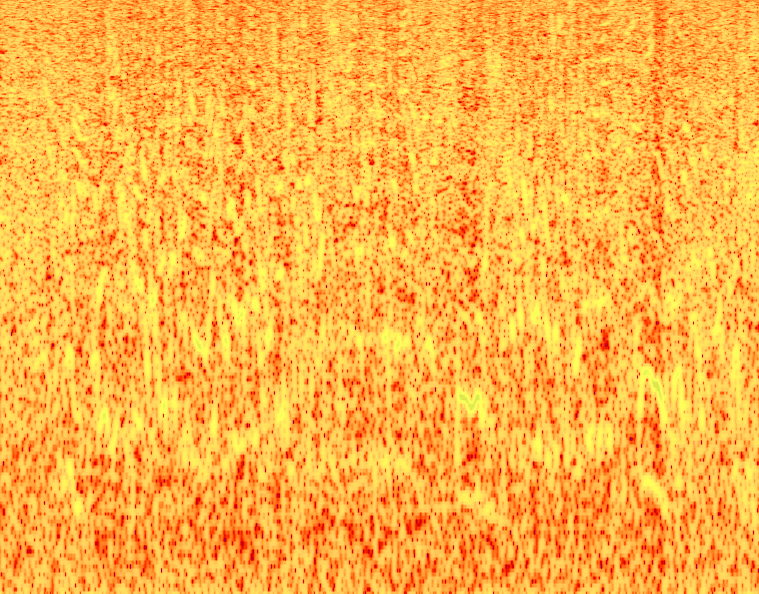
\includegraphics[width=0.40\textwidth]{figure/error-audio}
	\hspace{1cm}
	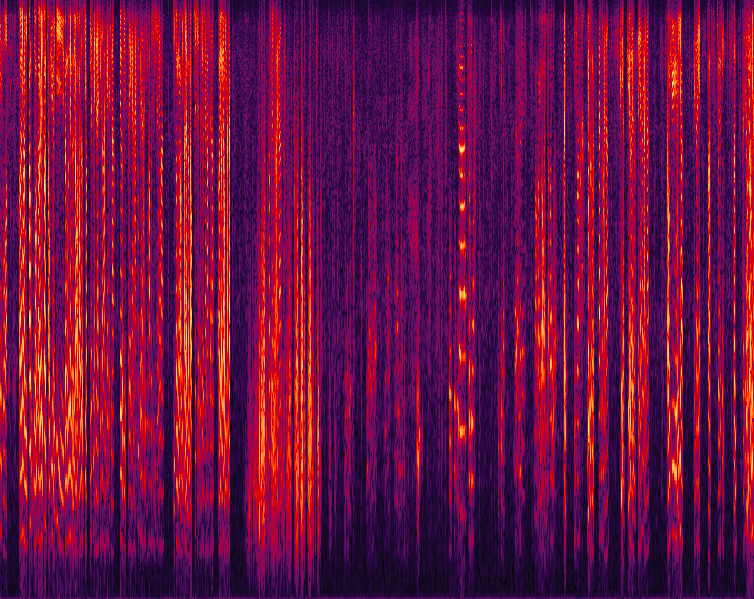
\includegraphics[width=0.40\textwidth]{figure/right-audio}
	\caption{损坏音频(左)与未损坏音频(右)频谱图}
\label{fig:audio-freq}
\end{figure}

损坏的音频听起来完全就是噪音,从频谱图上看整个频域信息有点类似于均匀分布,我们通过计算音频每一帧的RMS(Root-Mean-Square),结合每条音频的CER,交叉验证音频是否有效。RMS的计算如公式\ref{eqn:rms}。
\begin{align}
\label{eqn:rms}
	x_{\mathrm{RMS}}=\sqrt{\frac{1}{n}\left(x_{1}^{2}+x_{2}^{2}+\cdots+x_{n}^{2}\right)}
\end{align}

根据python处理音频的librosa库中所建议的,计算音频频谱值的RMS更为准确,所以再计算了音频每一帧的频谱值RMS之后,求整个音频的均值,通过观察损坏音频和未损坏音频的RMS均值,我们认定RMS均值6000以上且该句CER超过60\%的音频为无效音频,将其剔除。

剔除之后,我们进行了第二轮训练。

\subsection{第二轮训练过程及结果}
去除掉训练集和测试集中的无效数据之后,我们进行了第二轮的训练,训练的结果如表\ref{tab:second-train}所示。
\begin{table}[h]
 \centering
 \caption{2nd训练后不同LM下的测试结果}
	 \begin{tabular*}{1\textwidth}{@{\extracolsep{\fill}}ccccccc}
	 \toprule
		{\bf 语言模型} & {\bf 大小} & {\bf CE(\%)} &{\bf INS} &{\bf DEL}  &{\bf SUB} &{\bf Total}\\
	 \midrule
	   all-lm         &  83M   & 17.98   &  7410  &  9570  & 26886  & 243989 \\
	   small-lm       &  50M   & 24.04   &  9045  &   8707 & 40900  & 243989 \\
	   big-rescore-lm &  3.7G  & 22.97   &  8670  &   9244 & 37891  & 242932 \\
	 \bottomrule
	 \end{tabular*}%
 \label{tab:second-train}%
\end{table}%

而这个时候每个库的CER如表\ref{tab:second-each}。
\begin{table}[h]
 \centering
 \caption{2nd训练后不同库的CER}
	 \begin{tabular*}{1\textwidth}{@{\extracolsep{\fill}}ccccccc}
	 \toprule
		{\bf Project   } & {\bf ID   } & {\bf #WRDS   } & {\bf #SUB    } & {\bf #INS    } & {\bf #DEL    } & {\bf CER  } \\
	 \midrule
		TR2017097 &	005  &	15480   &	1596  &  	363    & 	440   &  	0.154974 \\
		TR2018011 &	011  &	5511    &	362   &  	89     & 	103   &  	0.100526 \\
		TR2018035 &	013  &	39569   &	4862  &  	1181   & 	1176  &  	0.182441 \\
		TR2018046 &	016  &	6889    &	713   &  	216    & 	235   &  	0.168965 \\
		TR2018063 &	018  &	5821    &	541   &  	109    & 	169   &  	0.140697 \\
		TR2018067 &	020  &	6959    &	1051  &  	416    & 	374   &  	0.264550 \\
		TR2018077 &	022  &	11382   &	626   &  	265    & 	344   &  	0.108505 \\
		TR2018086 &	025  &	2677    &	466   &  	98     & 	173   &  	0.275308 \\
		TR2018092 &	026  &	28489   &	4954  &  	1119   & 	1783  &  	0.275756 \\
		TR2018109 &	030  &	37833   &	4909  &  	811    & 	2194  &  	0.209182 \\
		TR2019068 &	044  &	17187   &	2193  &  	372    & 	635   &  	0.186187 \\
		kefu      &	049  &	66192   &	5275  &  	2040   & 	1613  &  	0.134880 \\
	 \bottomrule
	 \end{tabular*}%
 \label{tab:second-each}%
\end{table}%

\subsection{无关数据库测试}
为了验证最终训练出来的模型效果,我们选取了一些同类型的(客服或者电话)数据库进行识别测试。我们记录了不同数据库的识别结果,以及识别的时长。如表\ref{tab:other-corpus}。
\begin{table}[h]
 \centering
 \caption{2nd训练后模型之不相关数据测试}
	 \begin{tabular*}{1\textwidth}{@{\extracolsep{\fill}}ccccccc}
	 \toprule
		{\bf 数据库   } & {\bf 总时长   } & {\bf 识别时长   } & {\bf 未识别时长    } & {\bf CER    } & {\bf 类别    } \\
	 \midrule
		TR2018041 &     83.11  &    81.66  &     1.45&       32.58&       客服\/汽车 & \\
		TR2017115 &     270.31 &    270.31 &     0   &       35.99&       客服       & \\
		TR2017127 &     67.43  &    67.43  &     0   &       22.71&       客服       & \\
		TR2018012 &     112.69 &    112.69 &     0   &       24.04&       电话数据    & \\
		TR2018056 &     135.44 &    135.44 &     0   &       43.69&       电话数据\/分享报告& \\
		TR2018097 &     56.97  &    56.97  &     0   &       20.35&       客服/聊天   & \\
		TR2018119 &     345.24 &    345.24 &     0   &       19.22&       电话数据    & \\
		Total     &     1071.19&    ‬1069.74&‬     1.45&       27.87&      			 & \\
	 \bottomrule
	 \end{tabular*}%
 \label{tab:other-corpus}%
\end{table}%

对识别效果较差的数据库进行逐句分析,单句CER接近于1的音频识别差的原因有以下几点:
\begin{itemize}
	\item 音频为歌曲,文本为转写的歌词,如TR2017115中的部分数据;
	\item 音频在会场的环境录制,混响十分严重;
	\item 音频与文本不对应,即音频的参考文本是错的;
	\item 音频无对应的参考文本;
	\item 部分音频损坏,头文件包含的音频长度与实际音频长度不一致,导致参考文本中多出来很多无对应音频的segments;
	\item 部分方言很重的音频;
\end{itemize}

另外表格中未识别时长指的是模型未能识别的音频总时长,对这些音频进行分析,大部分都是问题音频,音频的长度接近于100或者200ms,参考的文本却有好多个字,这类音频因为太短,所以模型无法识别,故而跳过了。比如说下面这个音频片段,长度为63ms,对应的文本有30多个字。测试的这些库都存在这样的情况,表格中0是因为数量太少,所以直接就忽略了。
\begin{lstlisting}[language=shell, numbers=left, 
         numberstyle=\tiny,keywordstyle=\color{blue!70},
         commentstyle=\color{red!50!green!50!blue!50},frame=shadowbox,
         rulesepcolor=\color{red!20!green!20!blue!20},basicstyle=\ttfamily]
Index: 0170000000008-c2--1752605--1752668  
Time Length: 0.06299999999987449 
Text: 然后这位同事呢 他是做 的 当然知道什么样的东西不能做 但是经不住朋友的要求
\end{lstlisting}

\subsection{新语言模型解码结果}
新的语言模型大小为7.9 G,其发音词典有161460个词及其发音,词表有152946个词。其对应的小语言模型大小为165M,最终构图生成的G.carpa为9.3 G

\subsection{离线识别并输出timestamp}
选取了10000句短音频测试对齐效果,10000句的时长为17h,解码耗时10h,RTF=0.588(同样的数据和机器,另外一次解码耗时是6.75h,RTF=0.386)。解码输出的音素对齐如下所示:
\begin{lstlisting}[language=shell, numbers=left, 
         numberstyle=\tiny,keywordstyle=\color{blue!70},
         commentstyle=\color{red!50!green!50!blue!50},frame=shadowbox,
         rulesepcolor=\color{red!20!green!20!blue!20},basicstyle=\ttfamily]
[('SIL', 0, 6), ('du_B', 6, 2), ('ehH_I', 8, 2), ('iL_E', 10, 1), ('wu_B', 11, 1), ('oL_I', 12, 1), ('oL_I', 13, 1), ('m_I', 14, 1), ('elM_I', 15, 3), ('nnM_E', 18, 1), ('m_B', 19, 1), ('ehL_I', 20, 2), ('iH_I', 22, 2), ('yi_I', 24, 1), ('oL_I', 25, 1), ('uL_E', 26, 2), ('n_B', 28, 1), ('aH_I', 29, 2), ('aL_I', 31, 1), ('g_I', 32, 4), ('elM_I', 36, 1), ('elM_E', 37, 1), ('SIL', 38, 2), ('ji_B', 40, 2), ('iH_I', 42, 2), ('iH_I', 44, 1), ('ji_I', 45, 3), ('iH_I', 48, 2), ('nnH_E', 50, 4), ('SIL', 54, 9)]
\end{lstlisting}

其中每一个tuple代表的是音素、起始帧和该音素的帧长。kaldi中是基于堆叠多帧为一个大帧,然后跳帧输入的策略\upcite{subframe},stack 8帧,然后跳3帧,这样就不需要逐帧解码了,如图\ref{fig:subsample}而解码输出的时间是跳帧后的时间点,我们需要将其换算成对应的实际音频时间。
\begin{figure}[!ht]
	\centering
	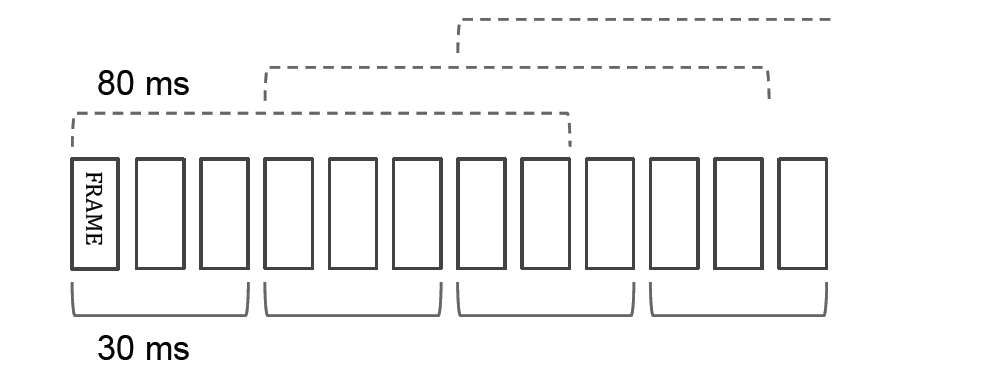
\includegraphics[width=0.8\textwidth]{subsample}
	\caption{stacking and subsampling of frames}
\label{fig:subsample}
\end{figure}

一帧所占时间长度为25ms,提取特征的时候帧移位10ms,一次stack的帧数为8帧,跳帧为3帧,设对齐音素的起始帧为$x$,帧数为$n$,那么我们可以通过公式\ref{eqn:compute-ali}得到该音素实际的起始时间$t_{s}$和结束时间$t_{e}$:
\begin{align}
\begin{split}
\label{eqn:compute-ali}
	t_{s} &= x*30 \\
	t_{e} &= (x+y)*30 \\
\end{split}
\end{align}

得到解码出的每个音素的timestamp之后,我们将其起止时间和标注的起止时间相减,得到每一个音频解码的对齐与实际标注的差异。10000句话的解码时间节点与标注的时间节点的起止时间差如图\ref{fig:ali-sta}和\ref{fig:ali-end}所示。
\begin{figure}[!ht]
	\centering
	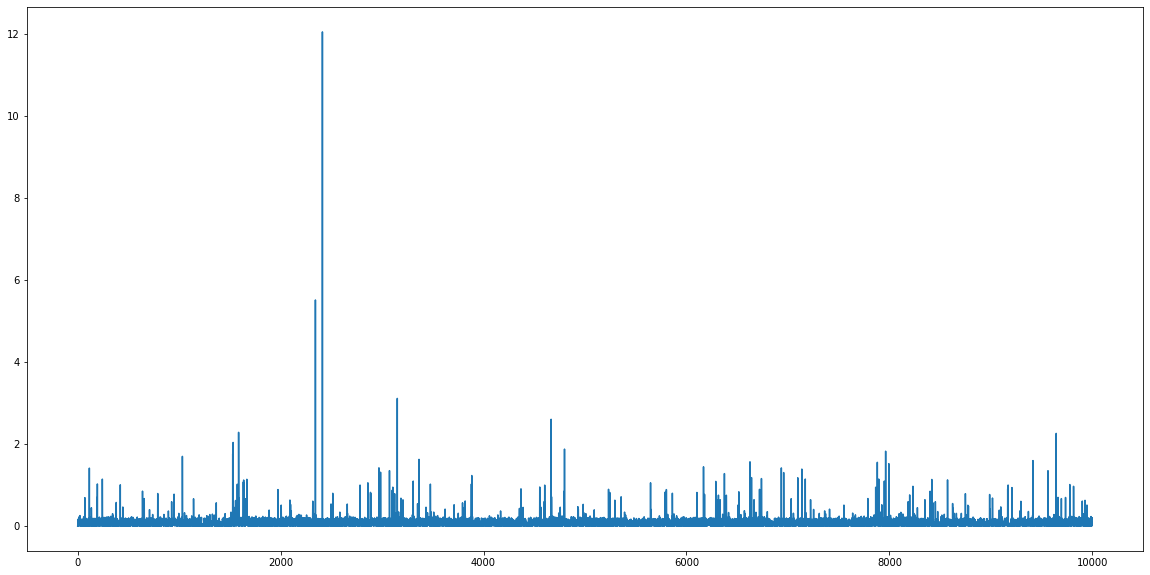
\includegraphics[width=0.8\textwidth]{ali-timestamp-start}
	\caption{解码和标注时间节点的起点时间差}
\label{fig:ali-sta}
\end{figure}

\begin{figure}[!ht]
	\centering
	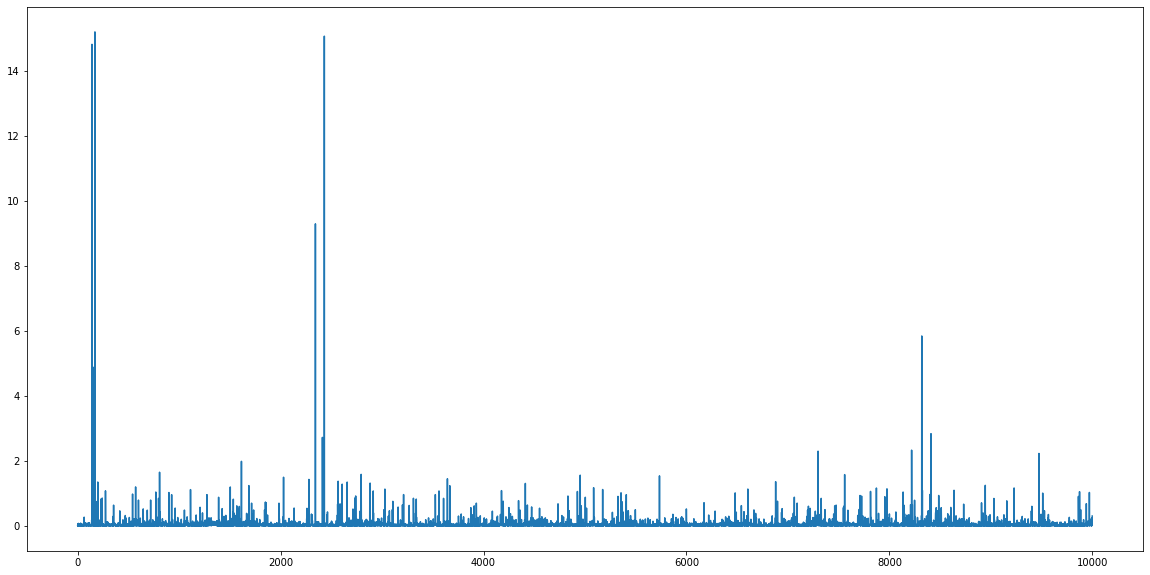
\includegraphics[width=0.8\textwidth]{ali-timestamp-end}
	\caption{解码和标注时间节点的终点时间差}
\label{fig:ali-end}
\end{figure}

对应差异在各个区间的分布如表\ref{tab:offline-dis}。

\begin{table}[h]
 \centering
 \caption{离线输出timestamp的误差分布}
	 \begin{tabular*}{1\textwidth}{@{\extracolsep{\fill}}cc}
	 \toprule
		{\bf 误差区间} & {\bf 比例} \\
	 \midrule
		(0.0, 0.1]   &  0.671833 \\
		(0.15, 0.2]  &  0.160902 \\
		(0.1, 0.15]  &  0.106536 \\
		(0.2, 0.3]   &  0.036090 \\
		(0.6, 1.0]   &  0.007519 \\
		(0.3, 0.4]   &  0.006131 \\
		(1.0, 15.0]  &  0.005784 \\
		(0.5, 0.6]   &  0.002660 \\
		(0.4, 0.5]   &  0.002545 \\
	 \bottomrule
	 \end{tabular*}%
 \label{tab:offline-dis}%
\end{table}%

\subsection{在线识别并输出timestamp}